\documentclass[journal]{IEEEtran}

\usepackage{graphicx}
\usepackage{hyperref}

\hypersetup{
    colorlinks=true,
    linkcolor=black,
    filecolor=black,      
    urlcolor=cyan,
    pdftitle={Computer Vision Chessboard},
    pdfpagemode=FullScreen,
    }

\usepackage[style=numeric]{biblatex}

\addbibresource{references.bib}

\newcommand\mkbibcolor[2]{\textcolor{#1}{\hypersetup{citecolor=#1}#2}}
\DeclareCiteCommand{\cite}[\mkbibcolor{black}]
  {\usebibmacro{prenote}}%
  {\usebibmacro{citeindex}%
   \usebibmacro{cite}}
  {\multicitedelim}
  {\usebibmacro{postnote}}

\begin{document}

% paper title
% can use linebreaks \\ within to get better formatting as desired
\title{Computer Vision Chessboard}

\author{Brandon~LeMay}

% make the title area
\maketitle

% As a general rule, do not put math, special symbols or citations
% in the abstract or keywords.
\begin{abstract}
The abstract goes here.
\end{abstract}

\begin{IEEEkeywords}
Chess, Computer Vision, OpenCV, Apriltag, Raspberry Pi.
\end{IEEEkeywords}


\section{Introduction}
\IEEEPARstart{C}{hessboards} as the subject of computer vision experiments are certainly nothing new. Blank chessboards are widely studied in computer vision both as methods to calibrate cameras, as chessboards have a very predictable geometry, so lens distortions are easy to counteract, and as a classic example for feature extraction, where a computer attempts to identify the distinct edges and corners of a chessboard in an image. [\cite{Forsyth2002}]

Many projects have also addressed the additional challenges of using computer vision to analyze a picture of a chessboard and return the types and positions of each piece on the board. Most of these, however, focus on taking a single image and converting it to 

% An example of a floating figure using the graphicx package.
% Note that \label must occur AFTER (or within) \caption.
% For figures, \caption should occur after the \includegraphics.
% Note that IEEEtran v1.7 and later has special internal code that
% is designed to preserve the operation of \label within \caption
% even when the captionsoff option is in effect. However, because
% of issues like this, it may be the safest practice to put all your
% \label just after \caption rather than within \caption{}.
%
% Reminder: the "draftcls" or "draftclsnofoot", not "draft", class
% option should be used if it is desired that the figures are to be
% displayed while in draft mode.
%
%\begin{figure}[!t]
%\centering
%\includegraphics[width=2.5in]{myfigure}
% where an .eps filename suffix will be assumed under latex, 
% and a .pdf suffix will be assumed for pdflatex; or what has been declared
% via \DeclareGraphicsExtensions.
%\caption{Simulation Results.}
%\label{fig_sim}
%\end{figure}

% Note that IEEE typically puts floats only at the top, even when this
% results in a large percentage of a column being occupied by floats.


% An example of a double column floating figure using two subfigures.
% (The subfig.sty package must be loaded for this to work.)
% The subfigure \label commands are set within each subfloat command,
% and the \label for the overall figure must come after \caption.
% \hfil is used as a separator to get equal spacing.
% Watch out that the combined width of all the subfigures on a 
% line do not exceed the text width or a line break will occur.
%
%\begin{figure*}[!t]
%\centering
%\subfloat[Case I]{
\includegraphics[width=2.5in]{box}%
%\label{fig_first_case}}
%\hfil
%\subfloat[Case II]{
\includegraphics[width=2.5in]{box}%
%\label{fig_second_case}}
%\caption{Simulation results.}
%\label{fig_sim}
%\end{figure*}
%
% Note that often IEEE papers with subfigures do not employ subfigure
% captions (using the optional argument to \subfloat[]), but instead will
% reference/describe all of them (a), (b), etc., within the main caption.


% An example of a floating table. Note that, for IEEE style tables, the 
% \caption command should come BEFORE the table. Table text will default to
% \footnotesize as IEEE normally uses this smaller font for tables.
% The \label must come after \caption as always.
%
%\begin{table}[!t]
%% increase table row spacing, adjust to taste
%\renewcommand{\arraystretch}{1.3}
% if using array.sty, it might be a good idea to tweak the value of
% \extrarowheight as needed to properly center the text within the cells
%\caption{An Example of a Table}
%\label{table_example}
%\centering
%% Some packages, such as MDW tools, offer better commands for making tables
%% than the plain LaTeX2e tabular which is used here.
%\begin{tabular}{|c||c|}
%\hline
%One & Two\\
%\hline
%Three & Four\\
%\hline
%\end{tabular}
%\end{table}


% Note that IEEE does not put floats in the very first column - or typically
% anywhere on the first page for that matter. Also, in-text middle ("here")
% positioning is not used. Most IEEE journals use top floats exclusively.
% Note that, LaTeX2e, unlike IEEE journals, places footnotes above bottom
% floats. This can be corrected via the \fnbelowfloat command of the
% stfloats package.

\section{Analysis of Applicable Standards}

\section{Theoretical Considerations}

\section{Work}

The computer vision program for monitoring the chessboard runs on a Raspberry Pi embedded in the frame of the chessboard. The program was written in Python, and can be split in three discrete sections: frame processing, where a picture of the chessboard is taken and analyzed to determine the position and color of each piece on the board. This information is then passed to the second section of the code that compares the current state of the board to the last state, and returns the move that was made to change the state of the board, if any. Lastly, another section of the code deals with peripherals meant to improve the user experience of the chessboard, including an animated representation of what the computer sees as the current board, and a custom PCB to control the chessboard, with buttons for starting, pausing, and stopping a game, as well as offering a draw or resigning.

\subsection{Physical Components and Construction}
A variety of manufacturing methods were used to create the physical chessboard, including milling, 3D printing, laser cutting, waterjet cutting, and sheet metal folding. The CAD model of the completed chessboard can be seen in Figure \ref{render}.


\begin{figure}[!ht]
	\centering
	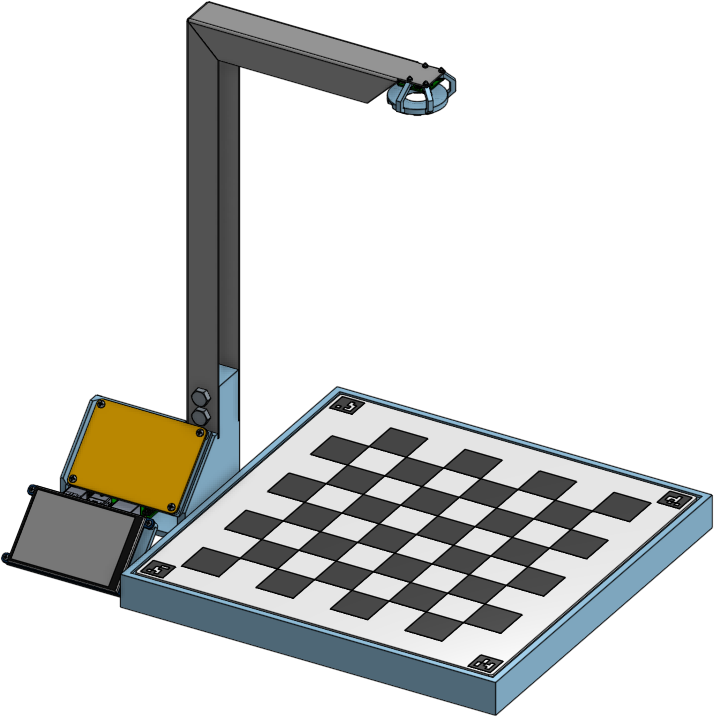
\includegraphics[width=\linewidth]{Images/Render.png}
	\caption{3D Render of CAD Model}
	\label{render}
\end{figure}

\vspace{12pt}

\subsubsection{PCB Milling}
A custom PCB was designed using EAGLE. The purpose of this circuit board is to provide a user interface that doesn't require a mouse or keyboard. A number of inputs were added to this PCB to communicate with the Raspberry Pi, including 5 buttons: 1 to start or pause a chess match, 1 to stop an ongoing match, 1 to toggle whether the user plays as white or black, 1 button for requesting a hint from a chess engine, and 1 button for offering a draw.

Figure \ref{PCB} shows the board design, the PCB has 2 copper layers, the red traces show the top layer, and blue denotes the bottom layer. Keen observers will note there is blue in the image than there is red, the bottom layer has a ground plane, so any "extra" copper not used for traces is connected to 0V.

\begin{figure}[!ht]
	\centering
	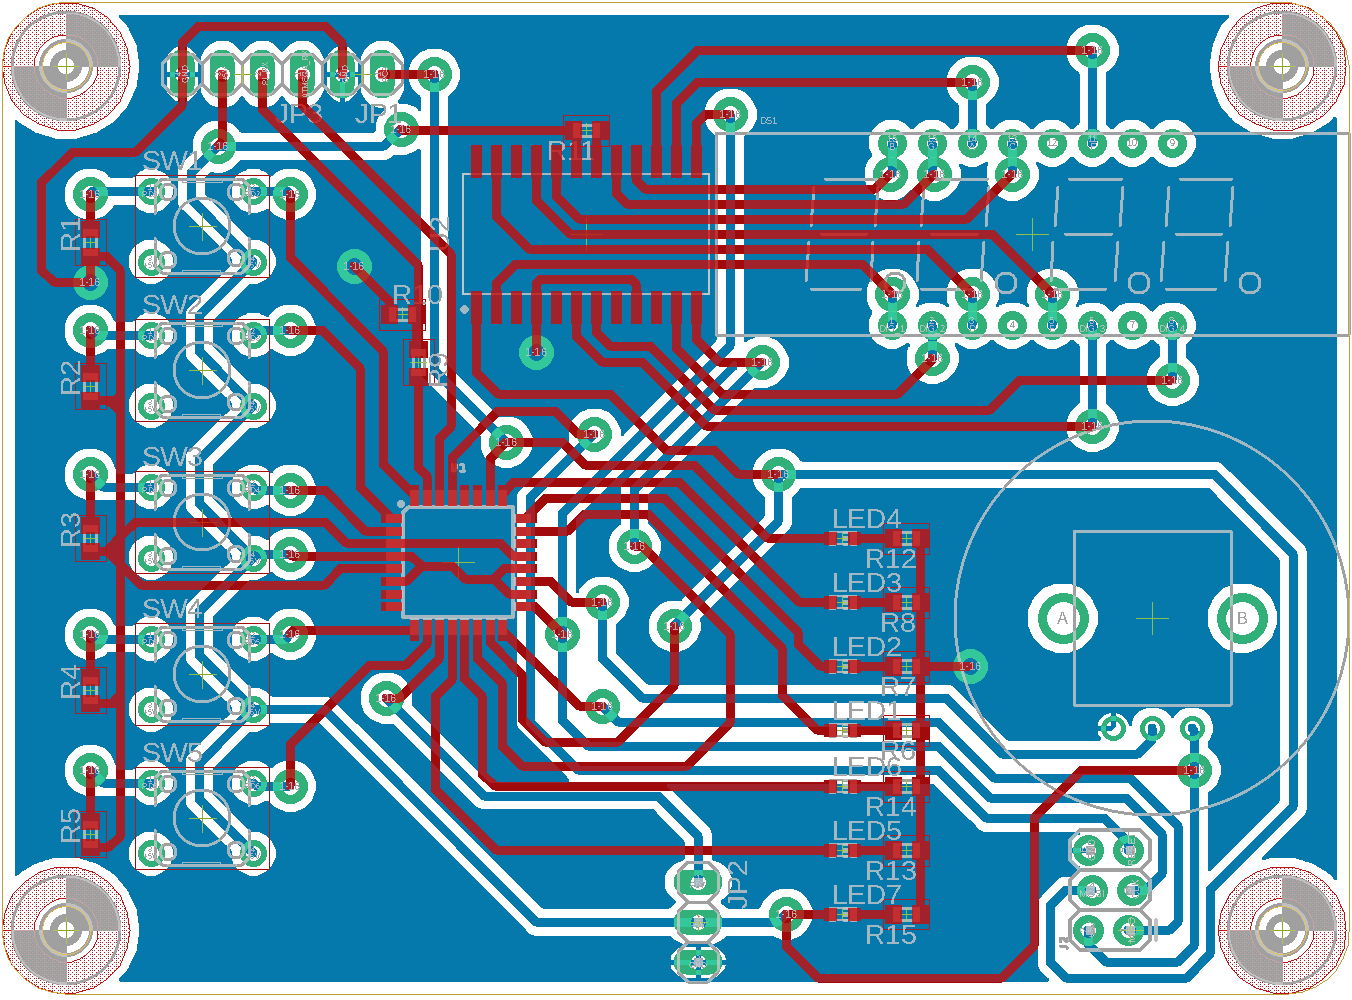
\includegraphics[width=\linewidth]{Images/ControlBoardDesign.png}
	\caption{Full Layer Stack of Control Board}
	\label{PCB}
\end{figure}

Also included are 6 controllable LEDs: 1 displays whether the user is playing as white or black, and the other 5 for signaling errors.
There is also another LED that automatially powers on when the circuit board is powered, this provides an easy way for the user to tell when the chessboard is powered.

To switch between the user playing another person and playing a computer, as well as selecting the skill of the computer, a potentiometer was added to the control board. The potentiometer has a detent in the middle of rotation, potentiometer positions to the counter-clockwise of the detent are for the user playing another human, with the position determining the skill of the chess engine providing hints. When the potentiometer is positioned on the detent, the chess engine is disabled and only move tracking is enabled for a more natural playing experience. When the potentiometer is positioned clockwise of the detent, the user plays against a chess engine, the rating of which is detemined by how clockwise the position is, more clockwise positions increase the skill of the chess engine.

Directly above the potentiometer is a 7-segment display that shows the rating of the chess engine, detemined by the potentiometer position. During gameplay, the display shows the move selected by the chess engine.

Lastly, three connectors are included on the board, one to power and control the LED ring around the camera that lights the chessboard, one to interface with the Raspberry Pi, and one to enable programming of the microcontroller on the PCB.

%\begin{figure}[!ht]
%	\centering
%	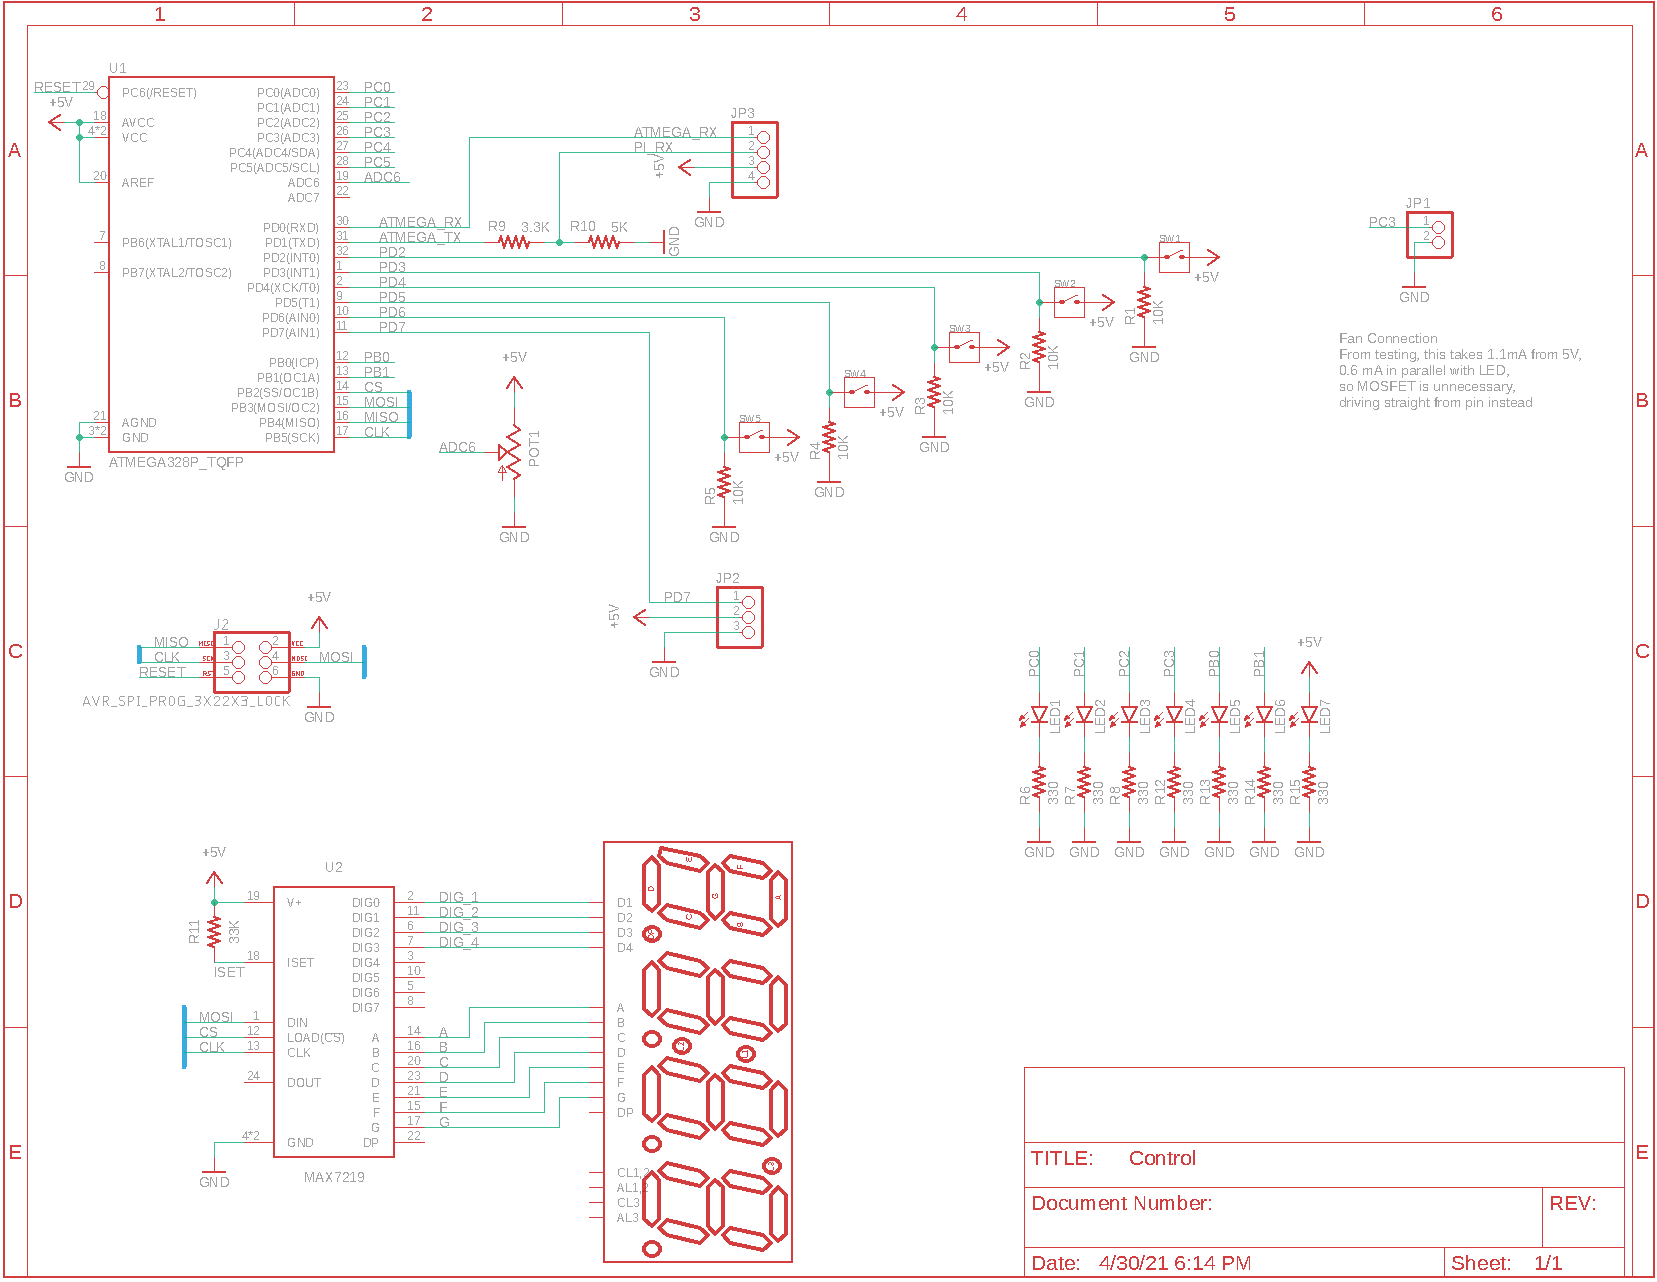
\includegraphics[width=\linewidth]{Images/ControlSchematicDesign.png}
%	\caption{Full Layer Stack of PCB}
%	\label{render}
%\end{figure}

To manufacture the circuit board, Gerber files were generated from the EAGLE design, which were then cut on an LPKF circuit board milling machine. A brass solder stencil was milled on an Othermill, and then used to apply solder paste to the pads of all the surface mounted devices (SMD). The SMD components were then placed on the board with tweezers, and the assembly was placed in a reflow oven to solder all SMD joints at once. Lastly, the remaining through-hole mounted (THM) components were placed and soldered by hand.

To program the ATMega328p on the circuit board that reads inputs from the buttons and potentiometers, communicates with the Raspberry Pi, and sets the display of the 7-segment display and LED ring, an AVR programmer was used. The code was written in C, compiled with avr-gcc, and written to the microcontroller using avrdude and a USBTiny ISP programmer

\vspace{12pt}

\subsubsection{3D Printing}
To compactly mount the Raspberry Pi, control PCB, and touchscreen display, and have user oriented components angled towards the user, exotic geometry was required. To easily fabricate these complex shapes, a Prusa MK3S FFM 3D printer was used.

Two important parts of the chessboard were 3D printed: the chessboard base that holds all the chess pieces when not in use and the chessboard sits on top of, and which the Raspberry Pi, control PCB, and touchscreen display all mount on. This base can be seen in Figure \ref{BoardMount}. 

\begin{figure}[!ht]
	\centering
	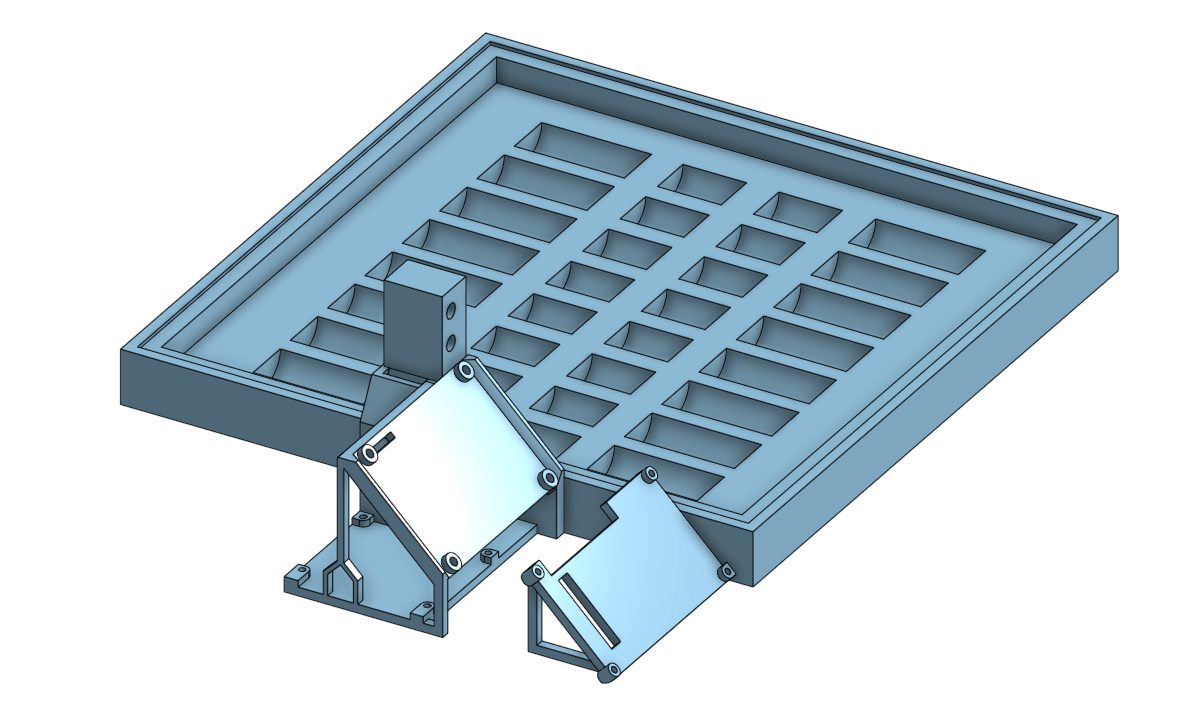
\includegraphics[width=\linewidth]{Images/BoardMount.png}
	\caption{Chessboard Base}
	\label{BoardMount}
\end{figure}

In addition, the LED light ring used to illuminate the chessboard is mounted to a 3D printed part that suspends it just below the camera to prevent it from blocking the cameras view while giving the light an unobstructed path to light up the chessboard. This standoff can be seen in Figure \ref{LEDMount}. 

\begin{figure}[!ht]
	\centering
	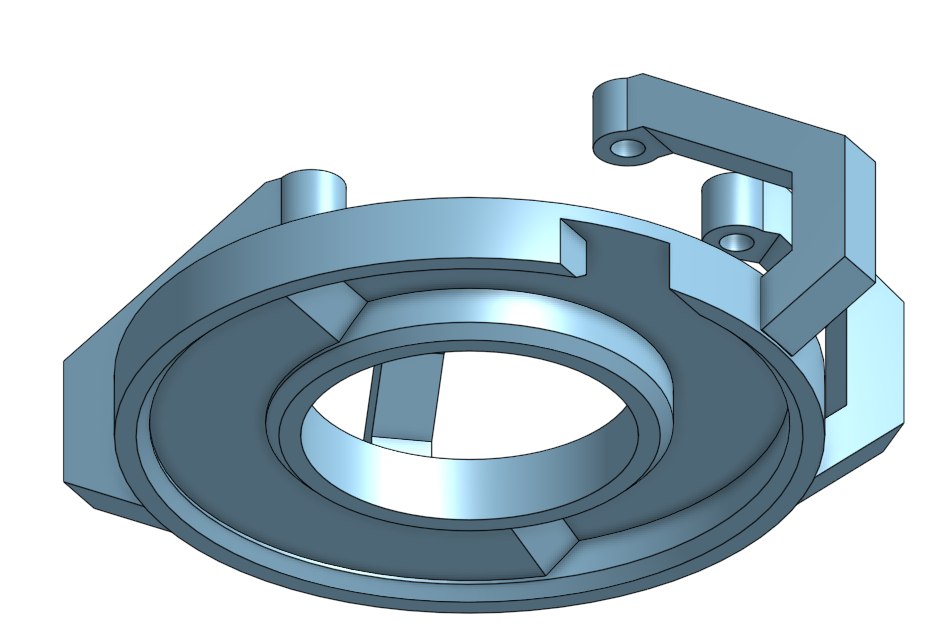
\includegraphics[width=\linewidth]{Images/LEDMount.png}
	\caption{LED Ring Light Mount}
	\label{LEDMount}
\end{figure}

The arms stretching above the circle set the mount just below the camera, while cutouts in the circle allow for wires to be soldered to the back of the LED ring and easily routed.

\vspace{12pt}

\subsubsection{Laser Cutting}

The wooden chessboard upon which the game is played was laser cut out of birch plywood, the interior of the board has the classic alternating pattern of colored squares that pieces are placed on, while the border of the board was reserved for image processing features. Apriltag fiducials were placed on each corner to assist in locating the chessboard in the frame of any image. Section \ref{ApriltagDetection} gives more information on this process. In between each tag, a Celtic knot pattern was placed, this design is used to tell when a user places their hand above the chessboard and obstructs the camera view. This feature is discussed more in Section \ref{ApriltagDetection}.

Figures \ref{input} and \ref{KnotCrop} show the chessboard from the perspective of the Raspberry Pi camera.

\vspace{12pt}

\subsubsection{Sheet Metal Forming}
To hold the camera above the chessboard, a crane was cut from aluminum sheet metal. Metal was used instead of plastic because the part was easily manufactured from flat panels, and provides more strength and rigidity, which is important to minimize blurring in images of the chessboard from the camera bouncing and flexing at the edge of the crane.

To make this part, the pattern shown in Figure \ref{CraneFlat} was cut on a waterjet cutter.

\begin{figure}[!ht]
	\centering
	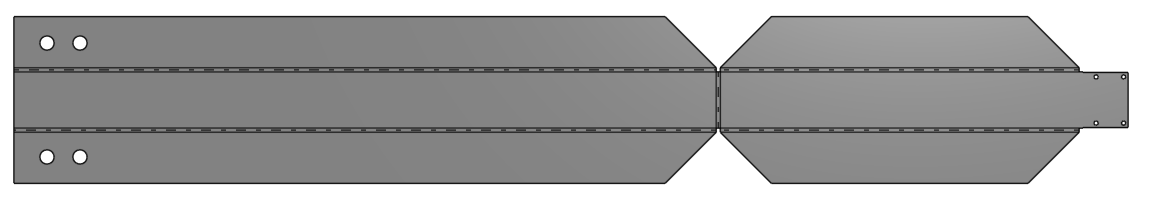
\includegraphics[width=\linewidth]{Images/CameraCraneFlat.png}
	\caption{Sheet Metal Crane Flat Pattern}
	\label{CraneFlat}
\end{figure}

This part was then folded on a sheet metal brake to form the shape shown in Figure \ref{Crane}.

\begin{figure}[!ht]
	\centering
	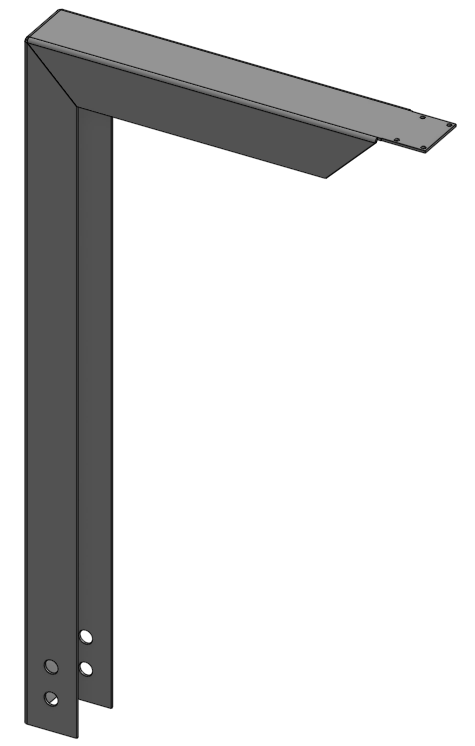
\includegraphics[width=0.7\linewidth]{Images/CameraCrane.png}
	\caption{Folded Sheet Metal Camera Crane}
	\label{Crane}
\end{figure}

This sheet metal crane fastens to the board mount shown in Figure \ref{BoardMount} using two large bolts, and the camera and LED ring mount onto the end of the crane using 4 M2.5 screws.

\vspace{12pt}

\subsection{Frame Processing}
The image processing component of the move tracking software can be split further into 4 sections: chessboard localization and cropping, obstruction testing, piece detection, and color detection. 

The program was designed with the assumption that the chessboard will not be in a fixed position in relation to the camera, and thus the first step for processing any frame is to find the location of the chessboard in the frame. Once the chessboard has been found, the corners of the chessboard are used to transform the image such that the rows and columns of the chessboard are horizontal and vertical in the frame of the image. As part of this transform, any area of the frame outside the chessboard is cropped.

After the chessboard has been located and transformed, the pattern on the edges of the board are compared to a template to make sure there is nothing obstructing the view of the chessboard from the camera. If any significant portion of the pattern is missing, then it is likely that a hand or arm is in the frame moving a piece, so the frame is thrown out and a new frame is taken.

Assuming no obstructions are detected, the frame is split into individual squares. These squares are then run through an edge detection algorithm to detect the amount of edges (sharp variations in color among nearly pixels) in the square. If the number of edges in a given square exceeds a certain threshold, the square is labelled as occupied.

Once each square has been labelled occupied or empty, the occupied squares are run through a color detecting function that converts the RGB image to HSV and uses the hue values of the square to determine what color the piece is, and thus can decide what side the piece belongs to.

Finally, an array containing both which squares are occupied and what color each of the pieces in an occupied square are is sent to the set of functions that parses what move was made, if any.

Figure \ref{input} shows an example of an input image. All the pieces are in their starting positions, and the edges of the chessboard are clearly visible, with no hands or arms reaching over the board to manipulate any pieces, thus this image should be processed as a valid image. This is the same input image used to derive most other images in this report, any visualizations not using this input image to start will be explicitly noted.

\begin{figure}[!ht]
	\centering
	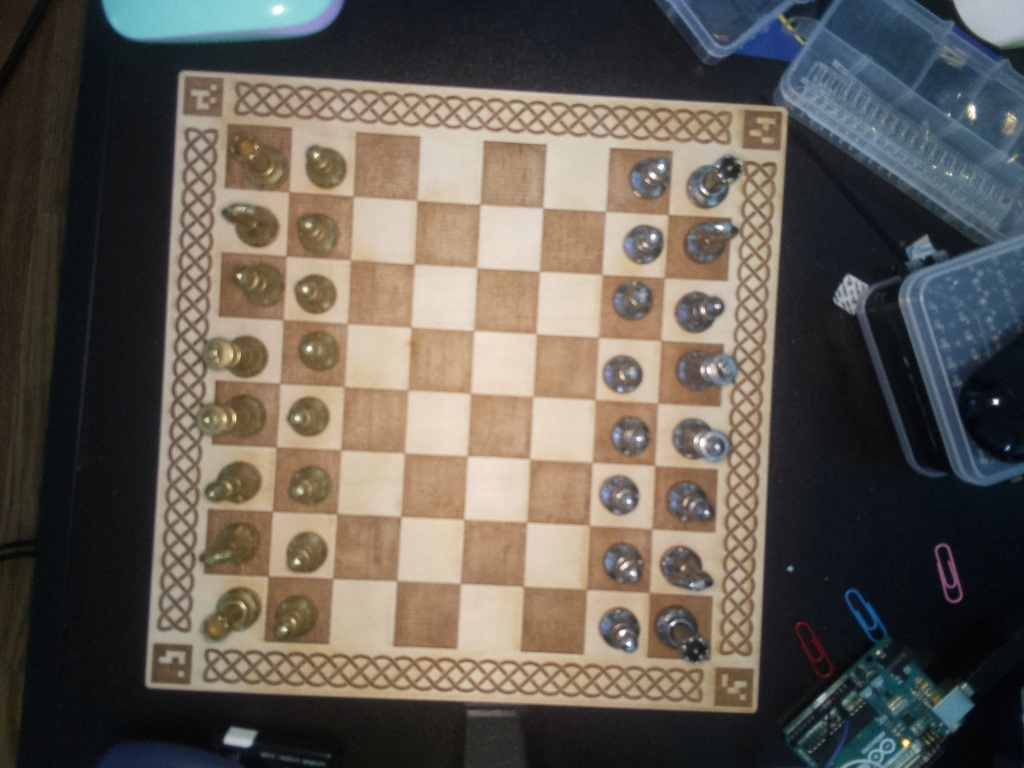
\includegraphics[width=\linewidth]{Images/InputImage.jpg}
	\caption{Input Image}
	\label{input}
\end{figure}

\vspace{12pt}

\subsubsection{Chessboard Localization}
\label{ApriltagDetection}
To determine where the chessboard is in the input frame, Apriltags were placed in each corner of the chessboard. Apriltags are a collection of unique two-dimensional patterns that can be easily detected using a camera, similar to a QR code, but much simpler in design to be easily recognized from a variety of distances [\cite{Wang2016}]. Each corner has an Apriltag with a different ID, which is recognizable by the computer when processing the image, thus the orientation of the chessboard can be kept constant.

To detect the Apriltags in the image, the python Apriltag library was used.
The tag detection was a significant bottleneck for the speed of the program, as the Raspberry Pi needs to determine the position of the chessboard in every frame, so running tag detection for every frame slowed down the processing time for each frame. To search the entire image for Apriltags took 762.9 milliseconds, in comparison, the rest of the image processing took a maximum of 500 seconds, so this delay in processing was significant.
%Check that processing time for the rest of the program
To decrease the time it takes to locate the chessboard, after the first frame is processed as normal, subsequent frames only search a small rectangle around where the tag was located in the previous frame. The time to find one Apriltag in one of these cropped search areas was 2.8 milliseconds, so the time to locate the chessboard was reduced to roughly 12 milliseconds, 63 times faster.

If the Apriltag detection algorithm returns a set of tags that doesn't contain the tags on the corners of the chessboard, the frame is ignored and another picture is taken to reexamine. The most likely reason for a tag not being included in the set of detected tags is because something is blocking the tag, so if there is an obstruction over any corner of the chessboard the frame can be thrown out without having to specifically test for any obstructions.

In order to be certain the Apriltags on the chessboard can be detected by the camera, the 16h5 tag family was chosen. This family of tags are all 4 pixel squares, the lowest amount of pixels per tag of any Apriltag family, allowing for each pixel to be larger than any other tag, meaning the tag is more likely to be detected.
This also means that it is easier for the Apriltag detection algorithm to return false positives, since each tag has less detail and thus non-tag objects or camera artifacts can appear to be valid tags by total chance. To remove these from consideration, the only detected tags that are used are tags that match the tag ID of the tags placed on the chessboard, and from those tags, only the 4 with the highest confidence are kept. Part of the information returned by the Apriltag detection algorithm is the confidence value for the tag, very clear tags have high confidence values, partially obstructed or blurry tags have low confidence values, thus by only keeping the tags with the 4 best confidence values, false positives are eliminated.

\vspace{12pt}

\subsubsection{Obstruction Testing}
\label{KnotDetection}

Once all 4 tags have been detected, the outside corners of the tags are used to reorient the perspective of the image. To do this, the image is transformed such that the pixel location representing the outside corner of each tag becomes the new corner of the image. Since the tags are equally spaced in each corner, this means that the horizontal rows of the chessboard are horizontal in the image, and the vertical columns are also vertical in the image. The outside corners are used to reorient the image so that the pattern going around the edges of the chessboard is visible, as can be seen in Figure \ref{KnotCrop}. 

\begin{figure}[!ht]
	\centering
	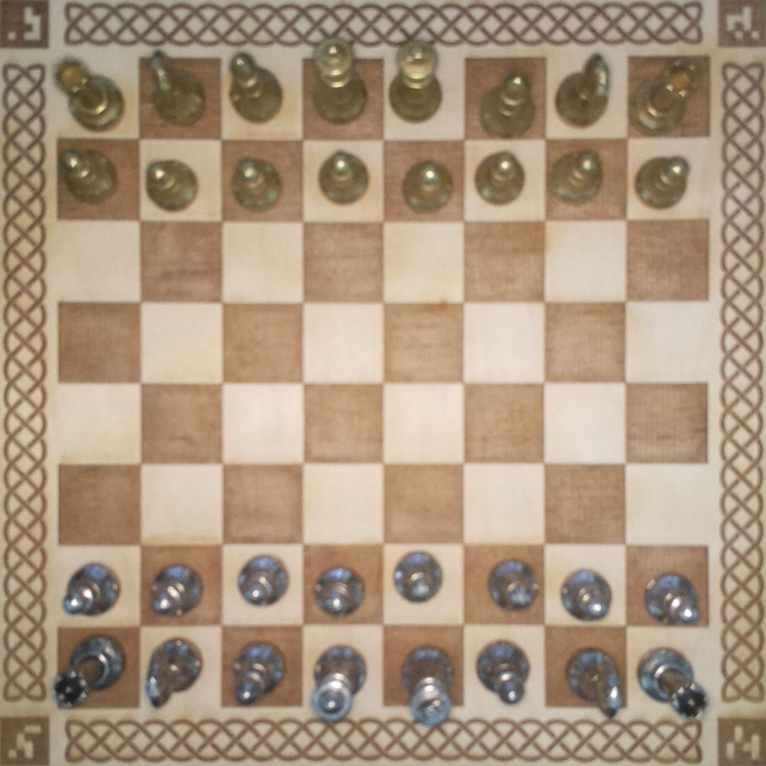
\includegraphics[width=\linewidth]{Images/InputImage_KnotCrop.jpg}
	\caption{Perspective Shifted Image}
	\label{KnotCrop}
\end{figure}

This knot pattern is used for testing whether a frame has an obstruction in it. For example, images where the user is moving a piece can't be used for image processing since the user's hand blocks the view of the camera. 
To detect whether this is the case, the detected edge pattern is compared to the pattern that was engraved onto the board.
This comparison is done by first scaling the template against which the detected pattern is to be compared to be the same size as the input image. Then, Canny edge detection is run on just the borders of the chessboard, excluding the inside of the board where all the squares are, as well as the corners of the board where the Apriltags are engraved.
The edges returned by the edge detection algorithm are then blurred to ensure that the pixels returned by the edge detection algorithm spread past just the edges of the pattern to fill the inside of each line.
An example of how this looks is given in Figure \ref{knot}, where these calculations are overlayed on the input image.

\begin{figure}[!ht]
	\centering
	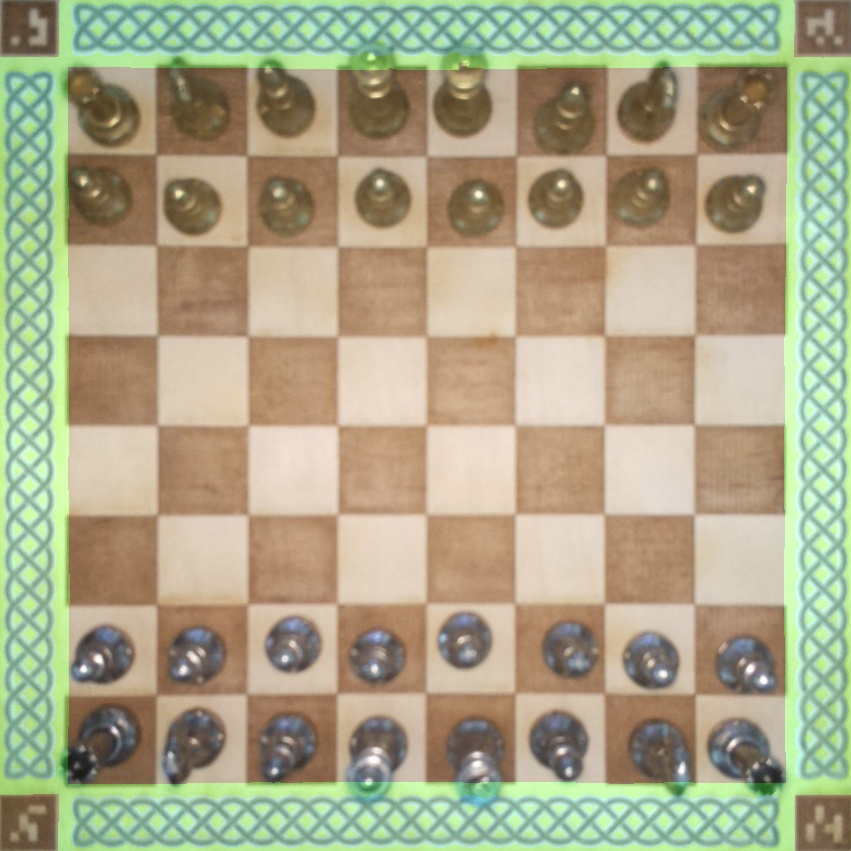
\includegraphics[width=\linewidth]{Images/KnotDetection.jpg}
	\caption{Obstruction Detection}
	\label{knot}
\end{figure}

The green blobs covering each edge are the blurred edge results, while the template to compare to are shown in blue.
Note that the blurring also acts to cover up small gaps missing from the pattern. In Figure \ref{knot} it is obvious to a human viewer that nothing is obstructing the camera's view of the chessboard, but close examination of the edge pattern would reveal small gaps where the perspective causes the king and queen pieces of both sides to cover up small portions of the pattern. But because the edge detection pixels are blurred, these small gaps are covered in green, which signifies that that portion of the pattern is considered accounted for.

To determine if there is an obstruction, the blurred edge matrix is subtracted from the template matrix. If the edges covers all portions of the template, this subtraction will result in zeros in every postition of the matrix. Any positive elements of the matrix are locations where the blurred edges don't cover the template. This implies that positive elements in the matrix resulting from taking the difference between the template and the blurred edges show areas where the camera is being obstructed.

This can be seen in Figure \ref{knot error}, where the green pixels again show the blurred edge matrix, and the template pattern is shown in blue, but any positive values of the difference matrix are shown in red.

\begin{figure}[!ht]
	\centering
	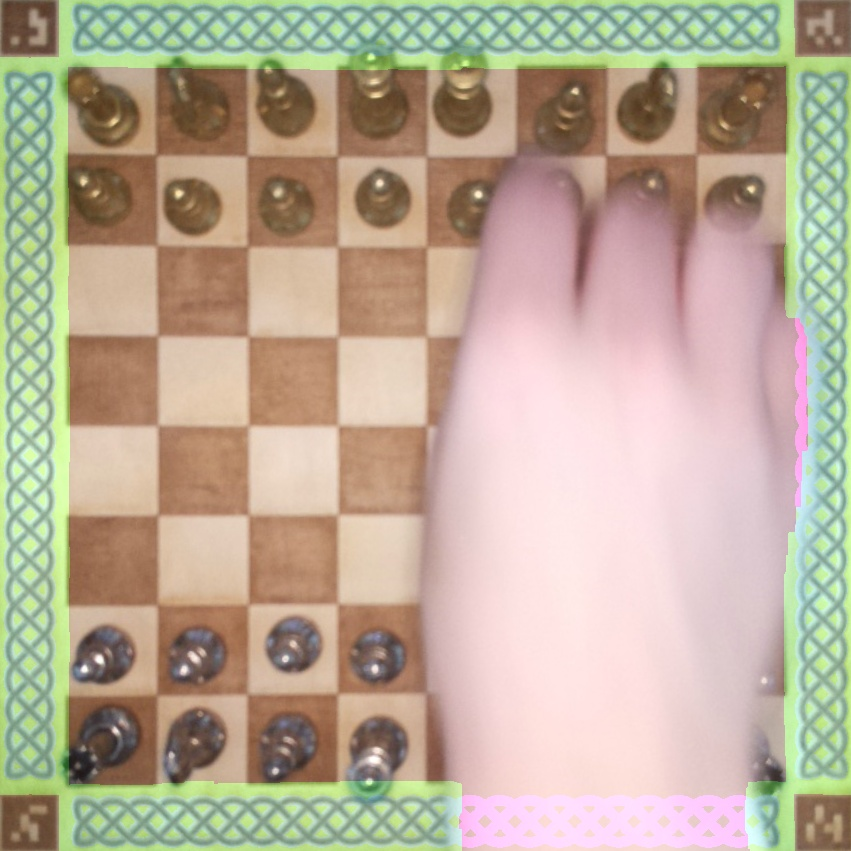
\includegraphics[width=\linewidth]{Images/KnotDetectionError.jpg}
	\caption{Obstruction Detection Error}
	\label{knot error}
\end{figure}

It is clear here that the wrist and the pinky both obstruct the edges of the chessboard, thus this image wouldn't be used image processing and another frame would be taken instead.

\vspace{12pt}

\subsubsection{Piece Detection}
Once the chessboard has been located and tested for obstructions, the program moves on to detecting where pieces are located on the chessboard.
Since pieces should be located within the bounds of each square of the chessboard, the first step in detecting the pieces is to split up the input image into individual squares.

To divide the image, first the image is cropped to get rid of the borders of the chessboard and just focus on the squares. To do this, the image is transformed such that the inside corners of each Apriltag becomes the corners of the image.
The perspective shifted image can be seen in Figure \ref{InsideCrop}.

\begin{figure}[!ht]
	\centering
	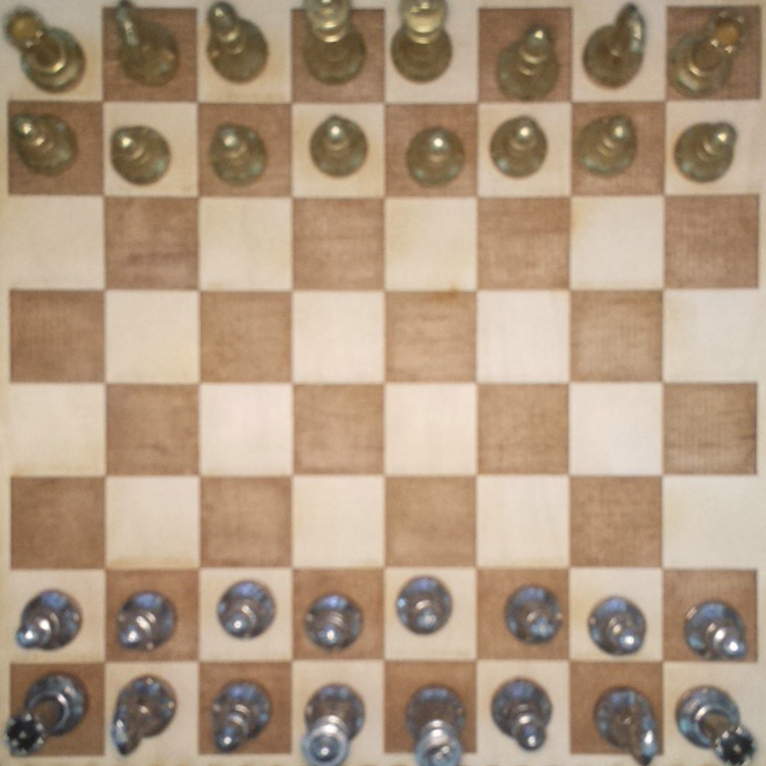
\includegraphics[width=\linewidth]{Images/InputImage_InsideCrop.jpg}
	\caption{Perspective Shifted Chessboard}
	\label{InsideCrop}
\end{figure}

The squares that are examined to determine if the square on the chessboard is occupied by a piece are all slightly smaller than the area of the square on the chessboard to create a border at the edge of each square that isn't used for piece detection. This border allows for pieces to be poorly placed or overlapping other squares without affecting the piece detection of nearby squares.

Figure \ref{piece zoomed} shows an example square of a populated square.

\begin{figure}[!ht]
	\centering
	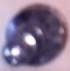
\includegraphics[width=\linewidth]{Images/KnotDetection340Zoomed.jpg}
	\caption{Single Occupied Square}
	\label{piece zoomed}
\end{figure}

The general idea to tell if a square is populated or not is to run Canny edge detection on the image of the square, then sum the number of edges detected. Figure \ref{piece detection zoomed} shows the result of Canny edge detection run on Figure \ref{piece zoomed}. The edge detection algorithm returns an array of ones and zeros, the zeros are shown as black pixels, and represent pixels from the original image that are not edges. The ones in the array are shown as white pixels, and represent pixels from the original image that are deemed edges.

\begin{figure}[!ht]
	\centering
	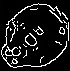
\includegraphics[width=\linewidth]{Images/PieceDetection340Zoomed.jpg}
	\caption{Single Square Piece Detection}
	\label{piece detection zoomed}
\end{figure}

If the total edge count of a square is greater than a predetermined threshold, then the square is deemed to be populated. The comparison threshold is automatically set from the data gathered in the first frame taken by the program. It assumes that the pieces will be in the starting position, and uses the average number of edges detected in the front and back two rows, where all the pieces start, to determine the average edge count of a populated square. The comparison threshold is then set to half the average value to account for lighting differences that might result in a piece blending in better with the board and returning less edges then average.

To help debug or diagnose errors, the program assembles all the single square images into the image shown in Figure \ref{piece detection}.

\begin{figure}[!ht]
	\centering
	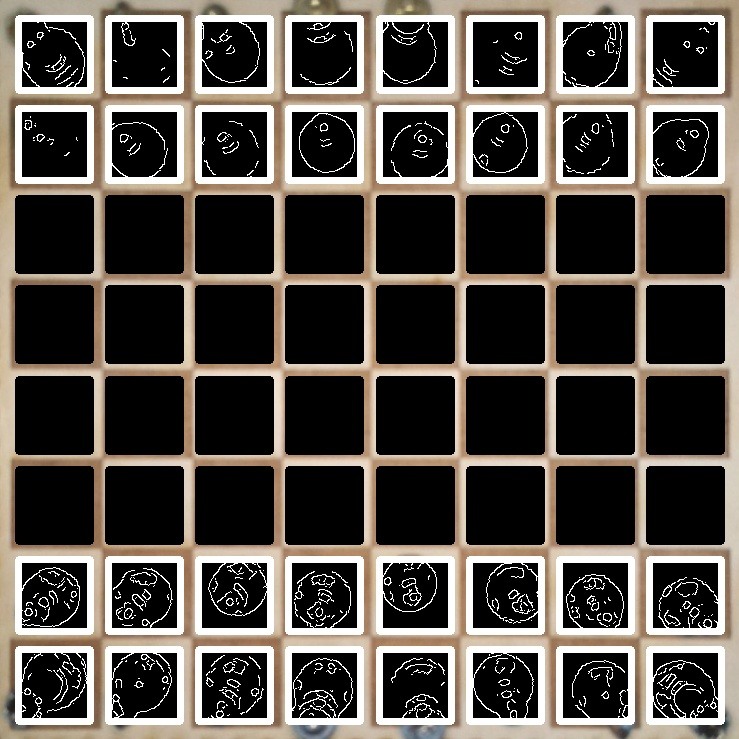
\includegraphics[width=\linewidth]{Images/PieceDetection.jpg}
	\caption{Full Board Piece Detection}
	\label{piece detection}
\end{figure}

All the single square images are superimposed on the board locations they were taken from, with a border added to show whether the square is occupied (the edge count of the square exceeds the comparison threshold) or not. White borders denote an occupied square, no borders denote an empty square.

\vspace{12pt}

\subsubsection{Color Detection}

\begin{figure}[!ht]
	\centering
	
\includegraphics[width=\linewidth]{Images/ColorDetection340Zoomed.jpg}
	\caption{Single Square Color Detection}
	\label{color zoomed}
\end{figure}

\begin{figure}[!ht]
	\centering
	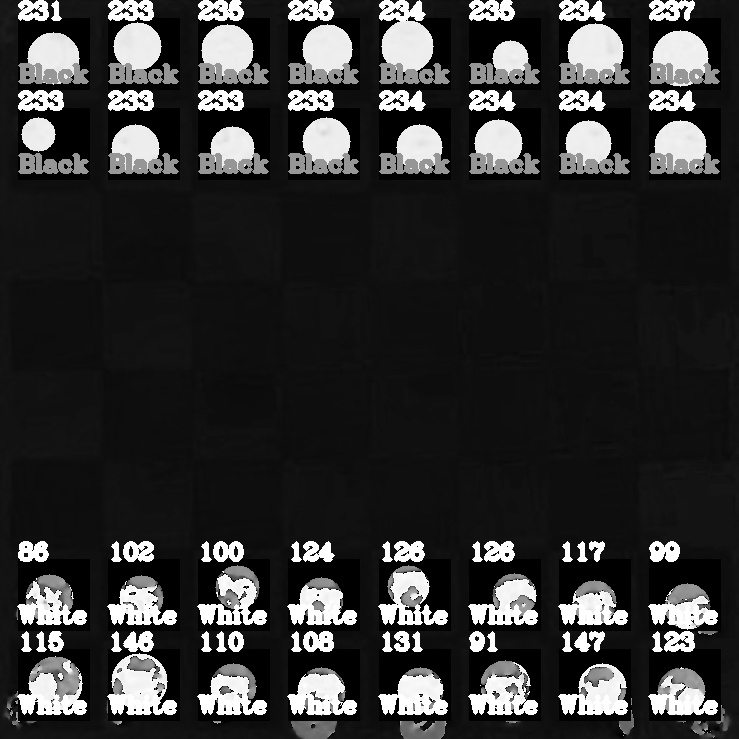
\includegraphics[width=\linewidth]{Images/ColorDetection.jpg}
	\caption{Color Detection}
	\label{color}
\end{figure}

\vspace{12pt}

\subsection{Parsing Detected Moves}

\section{Conclusions}

\section{Recommendations}
Correct for lens distortion/fisheye effect, the knot detection is a little distorted and doesn't always match the template near the edges of the board.

Save images of each square that has a piece on it to build up a database of correctly labeled pieces in order to train a machine learning algorithm to recognize piece types so promoted pieces can be automatically recognized.

Add mechanical actuators to move pieces automatically

Determine board orientation on first image, don't assume black side will be near certain apriltags

Generalize color determination settings to automatically work with any color

Add active lighting control to best enable piece and color detection

Rewrite knot detection to work with colors, not edges

% if have a single appendix:
%\appendix[Proof of the Zonklar Equations]
% or
%\appendix  % for no appendix heading
% do not use \section anymore after \appendix, only \section*
% is possibly needed

% use appendices with more than one appendix
% then use \section to start each appendix
% you must declare a \section before using any
% \subsection or using \label (\appendices by itself
% starts a section numbered zero.)
%


\appendices
\section{Code Repository}
The code for this project can be found here: \url{https://github.com/blemay360/Chessboard}

% you can choose not to have a title for an appendix
% if you want by leaving the argument blank
%\section{}
%Appendix two text goes here.

% Can use something like this to put references on a page
% by themselves when using endfloat and the captionsoff option.
\ifCLASSOPTIONcaptionsoff
  \newpage
\fi



% trigger a \newpage just before the given reference
% number - used to balance the columns on the last page
% adjust value as needed - may need to be readjusted if
% the document is modified later
%\IEEEtriggeratref{8}
% The "triggered" command can be changed if desired:
%\IEEEtriggercmd{\enlargethispage{-5in}}

% references section

\printbibliography

% that's all folks
\end{document}


